% ==============================================================================
% 3.1 DEFINICIONES INICIALES (FASE DE INICIO, PUDS)
% ==============================================================================
% [PENDIENTE]: Se proponen tres iteraciones; ajustar número y alcance (casos de uso por
% paquete, ver sección 3.2) y asociarlas a las fases Elaboración, Construcción y Transición.
% En esta versión no se usan historias de usuario (Scrum): la unidad de trabajo es el caso de uso.

\subsection{3.1. Definiciones Iniciales (Fase de Inicio)}

\subsubsection{3.1.1. Definir el equipo de desarrollo}

% [PENDIENTE]: Redactar "Definir el equipo de desarrollo".

\subsubsection{3.1.2. Definir el objetivo del producto}

El objetivo del producto corresponde al objetivo general del proyecto, presentado en la sección 1.5.2.1.

\subsubsection{3.1.3. Identificar los requerimientos iniciales}

Los requerimientos iniciales se detallan en los requisitos funcionales y no funcionales de la sección 3.2.3.

\subsubsection{3.1.4. Definir la duración de las iteraciones}

% [PENDIENTE]: Redactar "Definir la duración de las iteraciones".

\subsubsection{3.1.5. Definir la infraestructura tecnológica (hardware y software)}

% [PENDIENTE]: Redactar "Definir la infraestructura tecnológica (hardware y software)".

\subsubsection{3.1.6. Flujo de trabajo inicial}

% [PENDIENTE]: Redactar "Flujo de trabajo inicial".

\subsubsection{3.1.7. Modelos iniciales}

\paragraph{3.1.7.1. Contexto.}

El contexto del sistema es la organización para la cual se desarrolla: la Dirección Universitaria de Bienestar Social y Salud (DUBSS) de la UAGRM. A continuación se describen su identidad, su estructura organizacional, su ubicación e infraestructura, su modelo de negocio y su flujo operativo.

% [PENDIENTE]: Diagrama de contexto del sistema (actores externos y servicios: Firebase, módulo de IA).

% ------------------------------------------------------------------------------
% 3.1. DIRECCIÓN UNIVERSITARIA DE BIENESTAR SOCIAL Y SALUD (DUBSS)
% ------------------------------------------------------------------------------
\dbsa{\wn{3.1}. Dirección Universitaria de Bienestar Social y Salud (DUBSS)}\label{sec:empresa_general}

La Dirección Universitaria de Bienestar Social y Salud (DUBSS) es la unidad operativa central dependiente de la Universidad Autónoma Gabriel René Moreno (UAGRM) encargada de planificar, programar, coordinar y ejecutar acciones orientadas a mejorar la calidad de vida de la comunidad universitaria. Como órgano ejecutor del bienestar social, la DUBSS administra los programas de incentivos socioeconómicos y de salud integral, entre los cuales destaca la gestión del Comedor Universitario y la asignación del beneficio de Beca Comedor para los estudiantes en situación de vulnerabilidad.

La Dirección Universitaria de Bienestar Social y Salud (DUBSS) fue creada como una respuesta a la necesidad histórica de brindar asistencia integral a la comunidad universitaria de la UAGRM. A lo largo de los años, se ha consolidado como el pilar fundamental para garantizar la permanencia y graduación de los estudiantes con escasos recursos socioeconómicos, implementando programas emblemáticos como el Comedor Universitario, las Becas Trabajo, la guardería universitaria y el apoyo médico-psicológico. En la actualidad, la DUBSS afronta el reto de modernizar y digitalizar sus procesos de postulación e intensificar la transparencia en la adjudicación de sus beneficios sociales.

\dbsb{\wn{3.1}.1. Nombre}\label{sec:empresa_nombre}

\begin{itemize}
    \item \textbf{Nombre de la Institución:} Dirección Universitaria de Bienestar Social y Salud (DUBSS).
    \item \textbf{Entidad Superior:} Universidad Autónoma Gabriel René Moreno (UAGRM).
\end{itemize}

\dbsb{\wn{3.1}.2. Misión}\label{sec:empresa_mision}

La Dirección Universitaria de Bienestar Social y Salud (D.U.B.S.S.) es una unidad que contribuye al bienestar social de la población de la UAGRM, siendo el órgano que planifica, programa y coordina acciones orientadas a promover el desarrollo físico, mental, psicoafectivo, cognoscitivo y social de los estudiantes, docentes y administrativos.

\dbsb{\wn{3.1}.3. Visión}\label{sec:empresa_vision}

Ser una dirección que brinde servicio de calidez a la comunidad universitaria velando por el bienestar social, académico, cultural y deportivo de la población universitaria, proyectándose como una de las mejores direcciones de la universidad.

\dbsb{\wn{3.1}.4. Imagen Corporativa / Marca}\label{sec:empresa_marca}

La identidad visual de la DUBSS se encuentra alineada a la imagen institucional de la Universidad Autónoma Gabriel René Moreno (UAGRM), caracterizada por:

\begin{itemize}
    \item \textbf{Logotipo Institucional:} Emblema circular con el acrónimo DUBSS, integrado en conjunto con el escudo y la tipografía oficial de la UAGRM.
    \item \textbf{Colores Corporativos:} Azul institucional (que transmite confianza, seguridad y respaldo académico) y Rojo (asociado a la identidad y dinamismo de la UAGRM).
    \item \textbf{Posicionamiento:} Identificada por la comunidad estudiantil como el canal oficial de apoyo social, becas e incentivos universitarios.
\end{itemize}

\begin{figure}[H]
\caption{Logotipo institucional de la Dirección Universitaria de Bienestar Social y Salud (D.U.B.S.S.) de la UAGRM}
\label{fig:logo_dubss}
\centering

\includegraphics[width=0.4\linewidth]{images/002_Logo_DUBSS.jpg}

\smallskip
\noindent\raggedright\textit{Nota.} Recuperado del sitio web oficial de la DUBSS, de \url{https://dubs.uagrm.edu.bo/}
\end{figure}

\dbsb{\wn{3.1}.5. Web, Contacto, Redes Sociales}\label{sec:empresa_contacto}

\textbf{Sitio Web Oficial:} \url{https://dubs.uagrm.edu.bo/}

\begin{figure}[H]
\caption{Sitio web oficial de la Dirección Universitaria de Bienestar Social y Salud (DUBSS)}
\label{fig:web_dubss}
\centering

\includegraphics[width=0.85\linewidth]{images/010_PaginaWeb_DUBSS.jpg}

\smallskip
\noindent\raggedright\textit{Nota.} Captura de pantalla del sitio web institucional. Recuperado el 13 de septiembre de 2026, de \url{https://dubs.uagrm.edu.bo/}
\end{figure}

\textbf{Facebook:} \url{https://www.facebook.com/DireccionUniversitariaDeBienestarSocial}

\begin{figure}[H]
\caption{Página oficial de Facebook de la Dirección Universitaria de Bienestar Social y Salud (DUBSS)}
\label{fig:facebook_dubss}
\centering

\includegraphics[width=0.4\linewidth]{images/011_Facebook_DUBSS.jpg}

\smallskip
\noindent\raggedright\textit{Nota.} Captura de pantalla de la red social Facebook. Recuperado el 13 de septiembre de 2026, de \url{https://www.facebook.com/DireccionUniversitariaDeBienestarSocial}
\end{figure}

\textbf{Instagram:} \url{https://www.instagram.com/dubs_uagrm/}

\begin{figure}[H]
\caption{Perfil oficial de Instagram de la Dirección Universitaria de Bienestar Social y Salud (DUBSS)}
\label{fig:instagram_dubss}
\centering

\includegraphics[width=0.4\linewidth]{images/012_Instagram_DUBSS.jpg}

\smallskip
\noindent\raggedright\textit{Nota.} Captura de pantalla de la red social Instagram. Recuperado el 13 de septiembre de 2026, de \url{https://www.instagram.com/dubs_uagrm/}
\end{figure}


\textbf{Correo Electrónico:} dubs@uagrm.edu.bo

\textbf{Teléfono / WhatsApp de Atención:} +591 61537017


% ------------------------------------------------------------------------------
% 3.2. ESTRUCTURA ORGANIZACIONAL
% ------------------------------------------------------------------------------
\dbsa{\wn{3.2}. Estructura Organizacional}\label{sec:estructura_organizacional}
% [INSTRUCCIÓN]: Organigrama, roles, áreas funcionales y responsabilidades del equipo de trabajo.

\begin{figure}[H]
\caption{Organigrama de la Dirección Universitaria de Bienestar Social y Salud (DUBSS)}
\label{fig:organigrama_dubss}
\centering
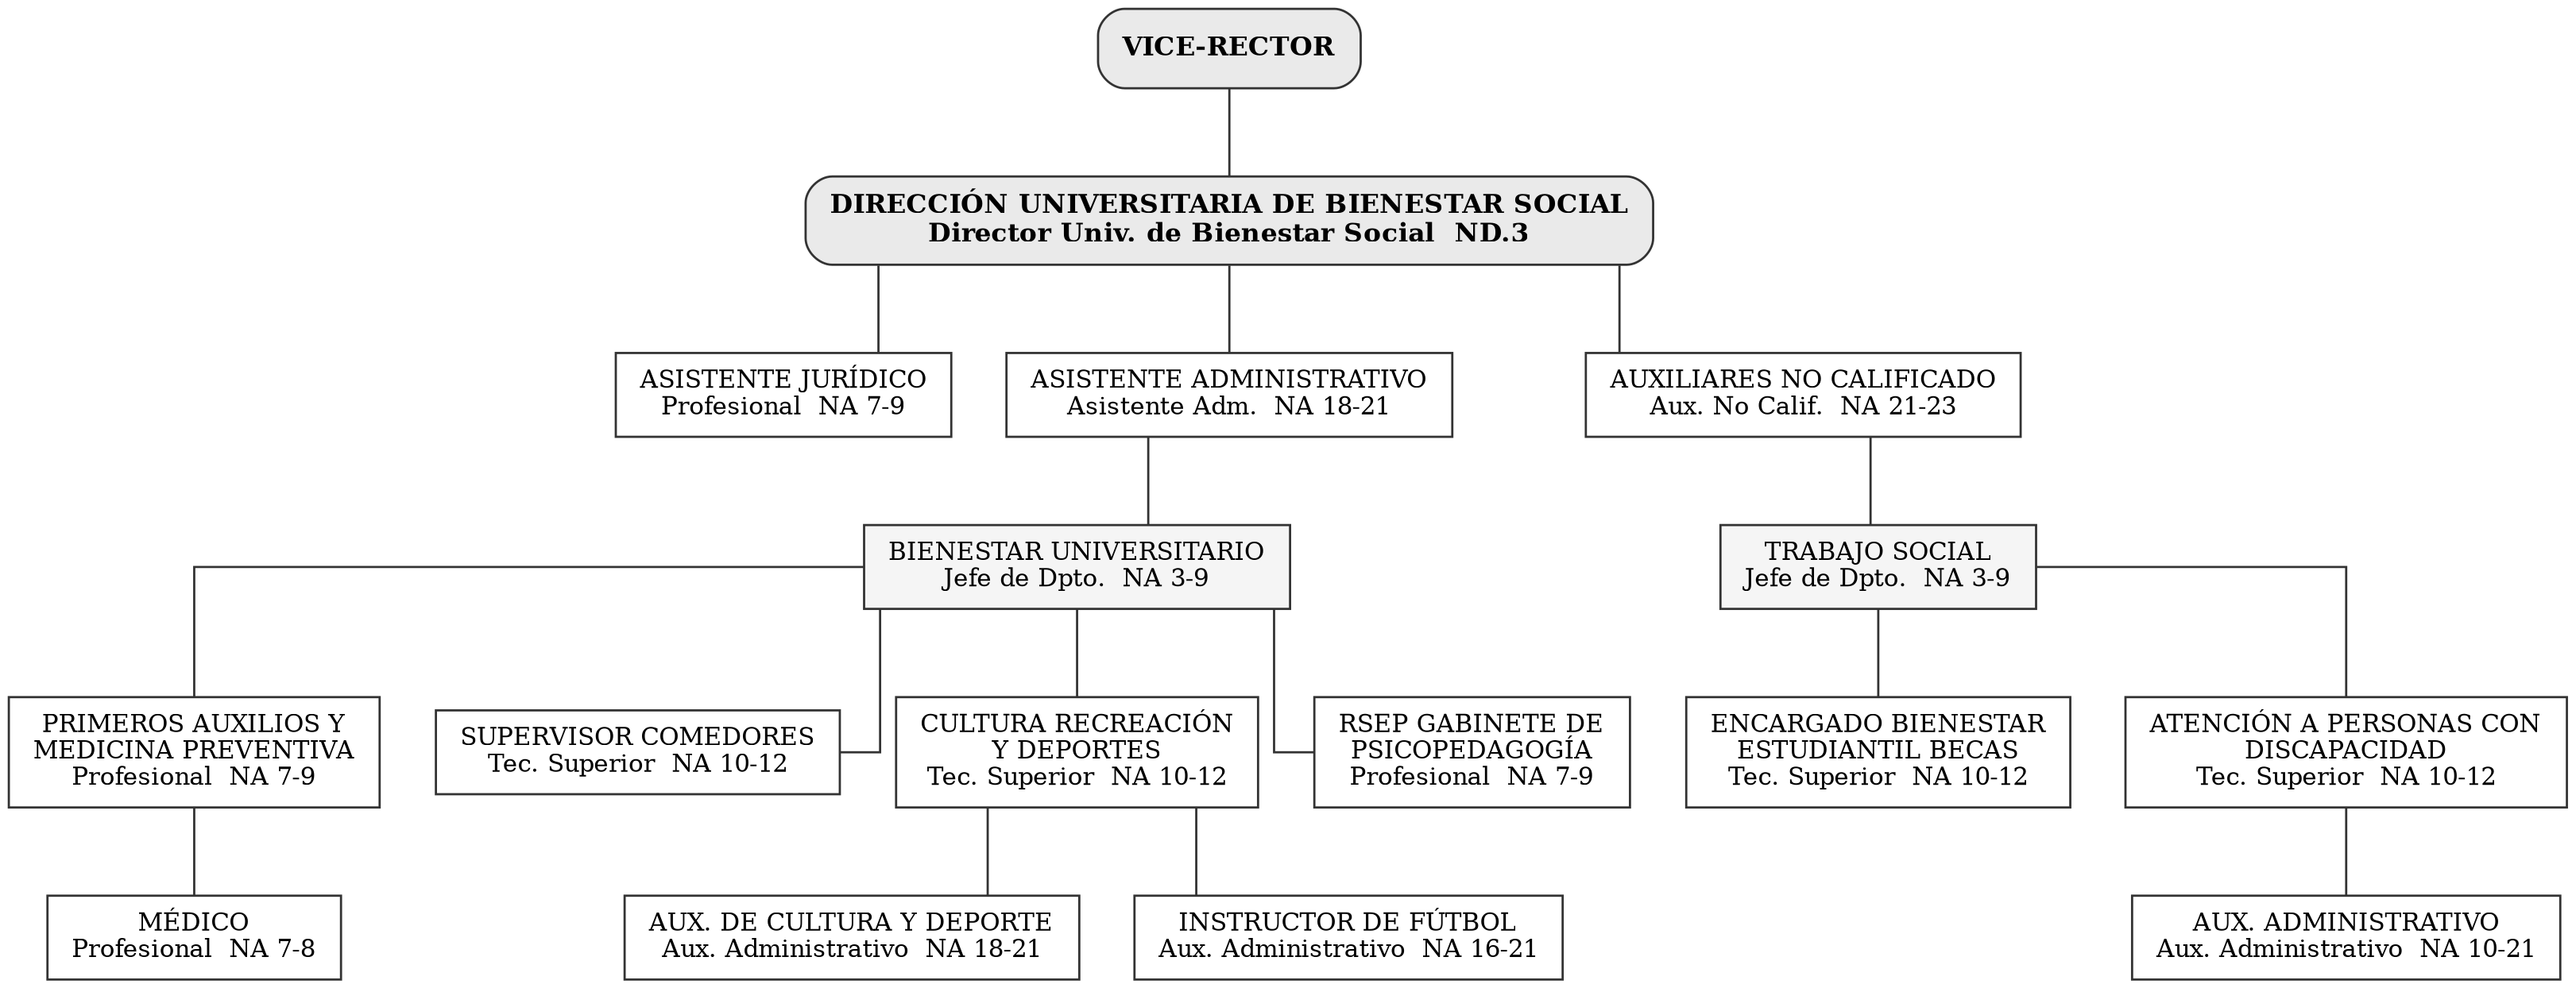
\includegraphics[width=\textwidth]{images/005_Organigrama_DUBSS.png}

\smallskip
\noindent\raggedright\textit{Nota.} Elaboración propia en base a los datos institucionales de la DUBSS.
\end{figure}

\clearpage
% ------------------------------------------------------------------------------
% 3.3. UBICACIÓN E INFRAESTRUCTURA
% ------------------------------------------------------------------------------
\dbsa{\wn{3.3}. Ubicación e Infraestructura}\label{sec:ubicacion_infraestructura}
% [INSTRUCCIÓN]: Ubicación geográfica de la sede operativa, centros de datos y facilidades técnicas.

\begin{figure}[H]
\caption{Comedor Universitario de la Universidad Autónoma Gabriel René Moreno}
\label{fig:comedor_universitario}
\centering

\includegraphics[width=0.5\textwidth]{images/006_Comedor_Universitario.jpeg}

\smallskip
\noindent\raggedright\textit{Nota.} Elaboración propia.
\end{figure}

\begin{figure}[H]
\caption{Oficinas de la Dirección Universitaria de Bienestar Social y Salud (DUBSS)}
\label{fig:oficinas_dubss}
\centering
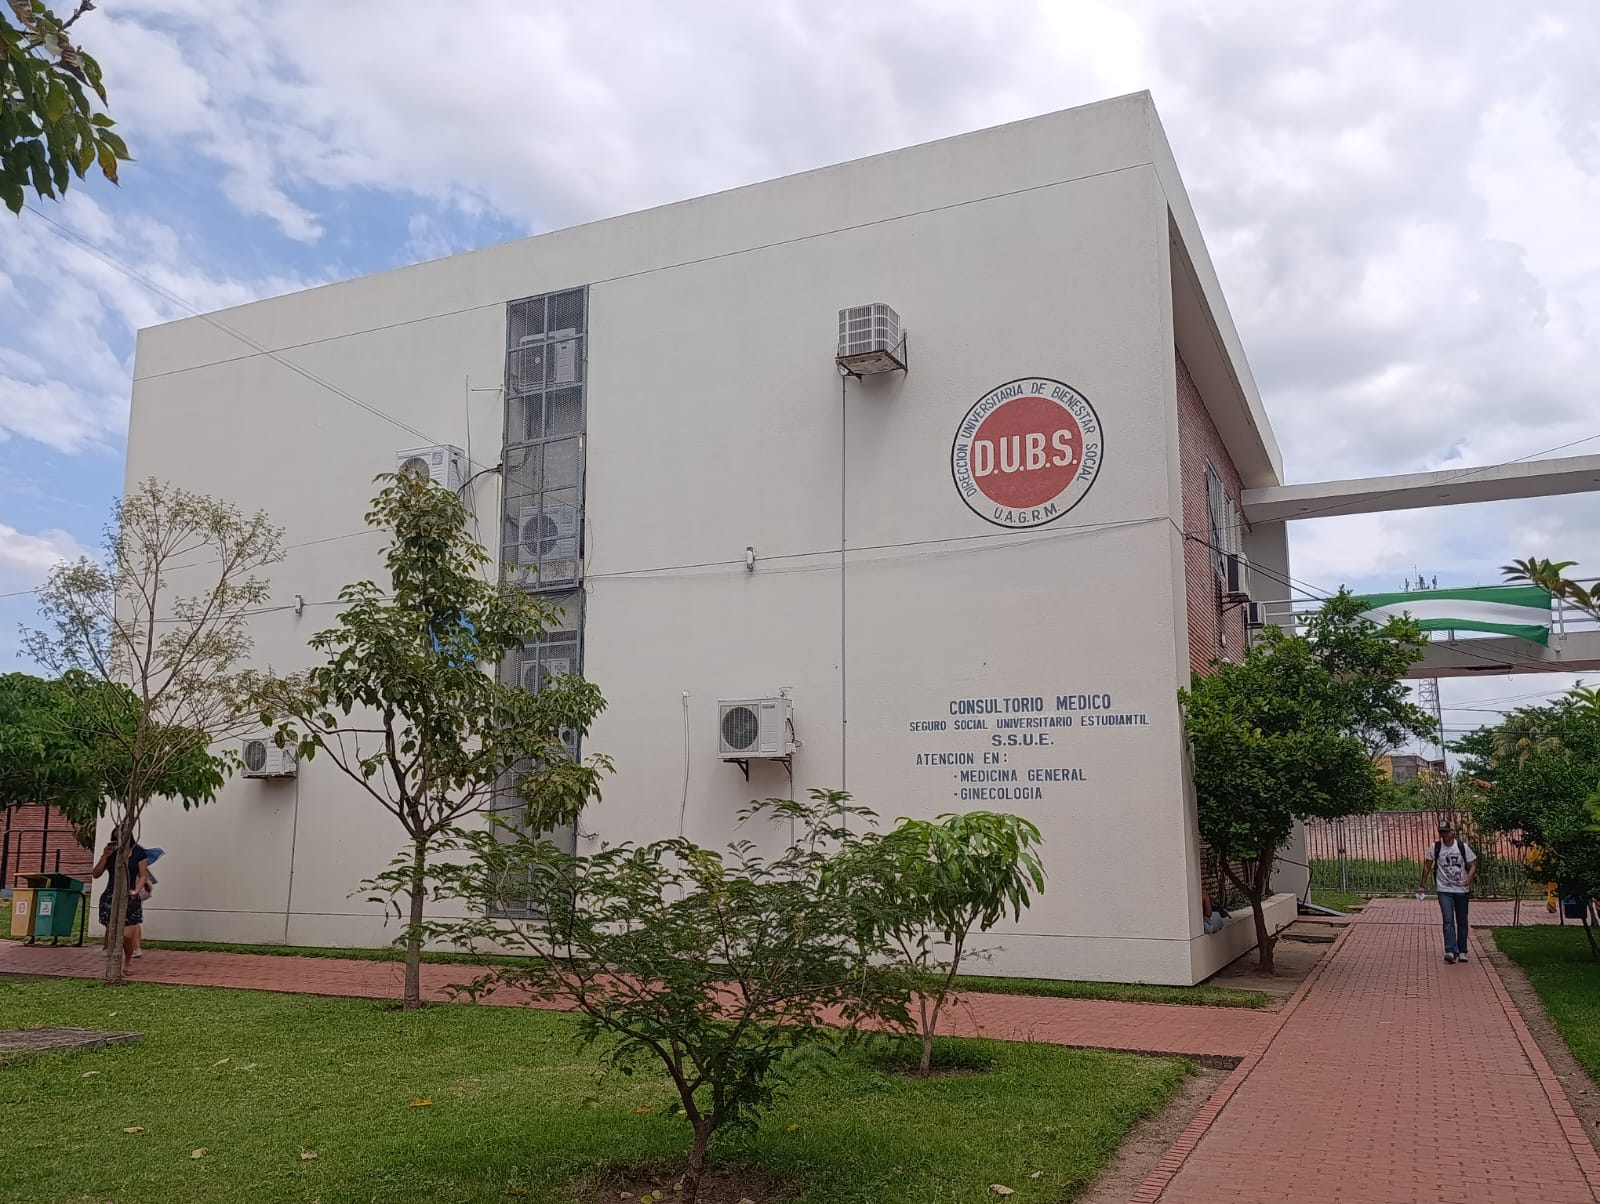
\includegraphics[width=0.5\textwidth]{images/007_Oficinas_DUBSS.jpeg}

\smallskip
\noindent\raggedright\textit{Nota.} Elaboración propia.
\end{figure}

\clearpage
\begin{figure}[H]
\caption{Ubicación de las instalaciones de la DUBSS en el campus universitario}
\label{fig:ubicacion_dubss}
\centering
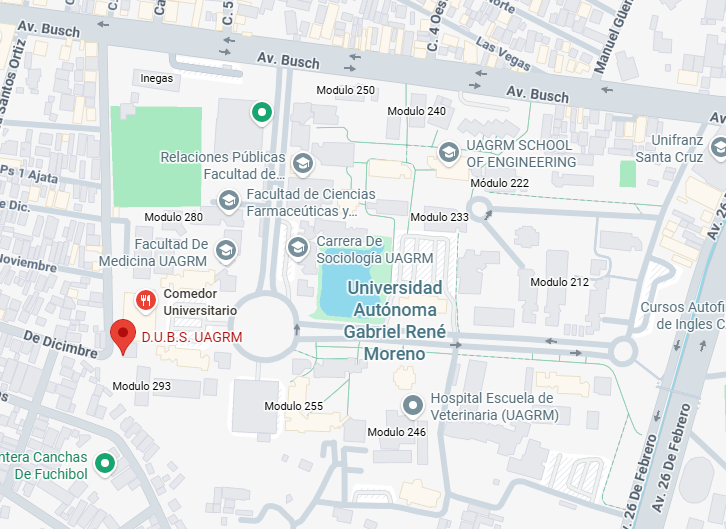
\includegraphics[width=\textwidth]{images/008_Ubicacion_DUBSS.png}

\smallskip
\noindent\raggedright\textit{Nota.} Elaboración propia a partir de una captura de Google Maps.
\end{figure}

% ------------------------------------------------------------------------------
% 3.4. MODELO DE NEGOCIO
% ------------------------------------------------------------------------------
\dbsa{\wn{3.4}. Modelo de Negocio}\label{sec:modelo_negocio}
% [INSTRUCCIÓN]: Propuesta de valor, segmentos de clientes, fuentes de ingresos y esquema de sostenibilidad (lienzo Canvas si aplica).

\begin{figure}[H]
\caption{Modelo de negocio propuesto para el Sistema de Información de la Beca Comedor}
\label{fig:modelo_negocio}
\centering
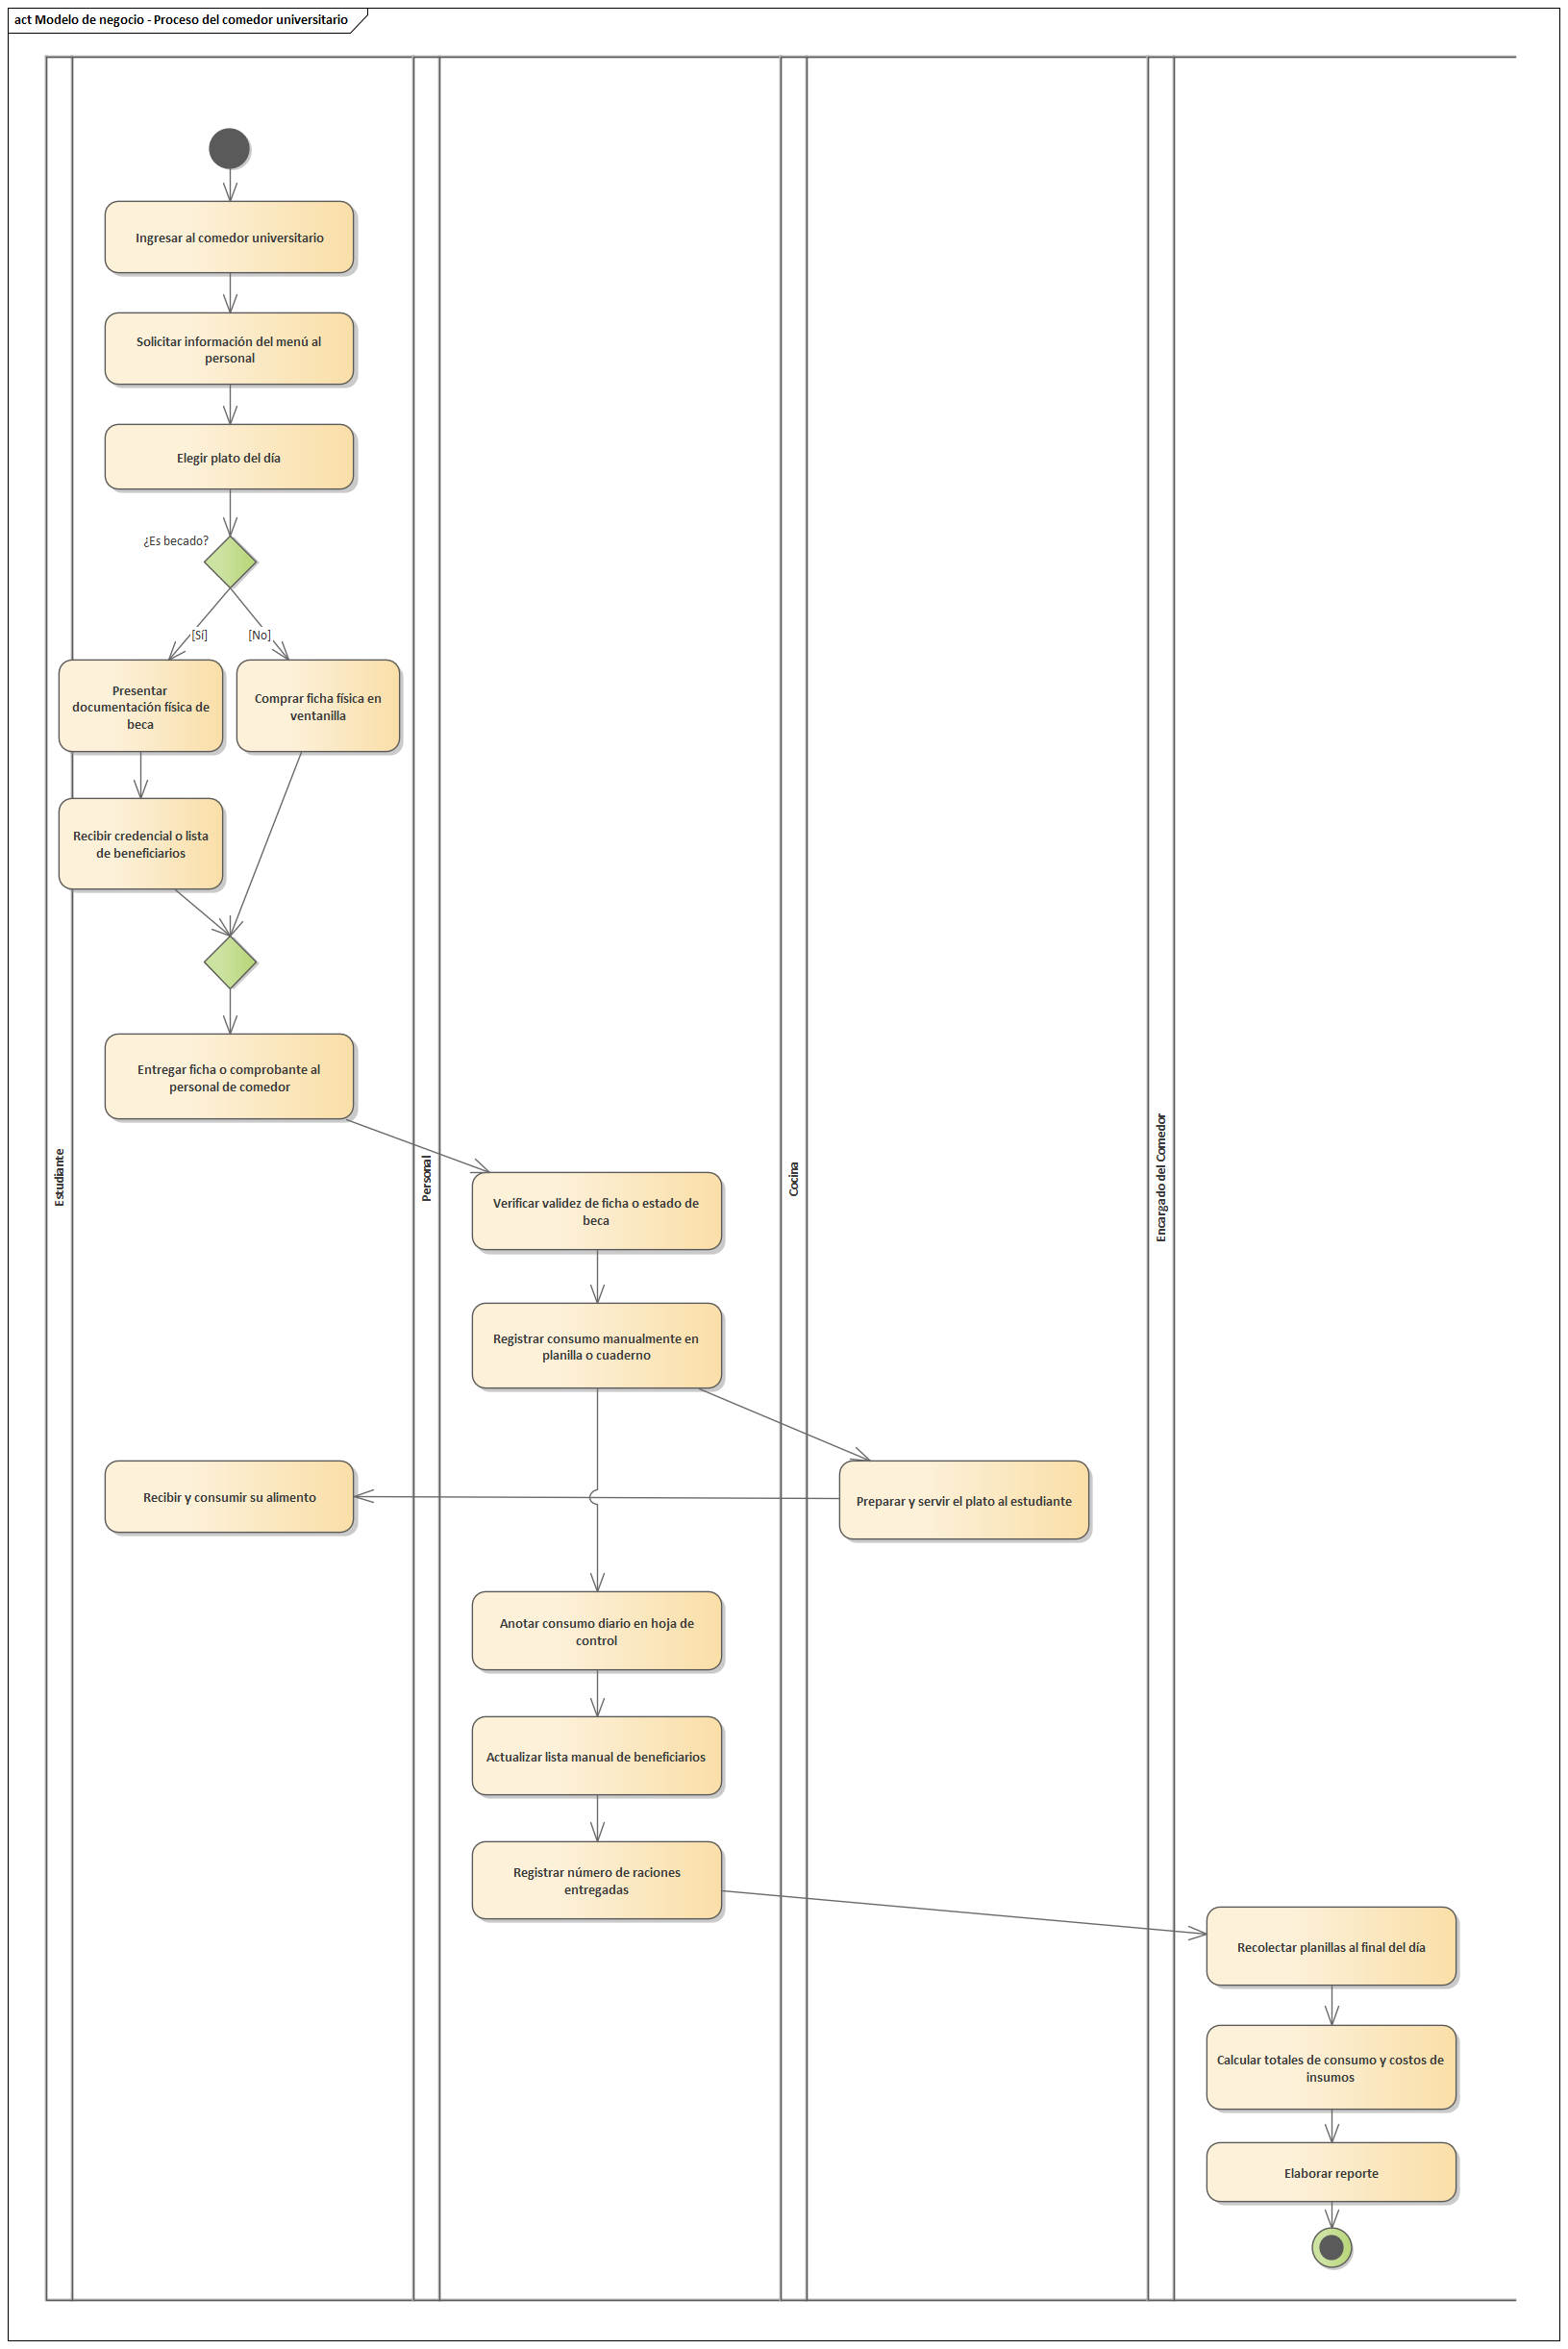
\includegraphics[width=\textwidth,height=0.78\textheight,keepaspectratio]{images/009_Modelo_Negocio.png}

\smallskip
\noindent\raggedright\textit{Nota.} Elaboración propia con información de la DUBSS.
\end{figure}

% ------------------------------------------------------------------------------
% 3.5. FLUJO OPERATIVO
% ------------------------------------------------------------------------------
\dbsa{\wn{3.5}. Flujo Operativo}\label{sec:flujo_operativo}

El flujo operativo describe cómo se desarrolla actualmente, en la Dirección Universitaria de Bienestar Social y Salud (DUBSS), el proceso de postulación y adjudicación de la Beca Comedor. En él intervienen el postulante, que presenta su carpeta con la documentación de respaldo; el personal de Trabajo Social, que revisa los documentos y califica la solicitud; y la Encargada de Sistemas, que incorpora el rendimiento académico y calcula el puntaje total que determina la adjudicación. La Figura~\ref{fig:postulacion_beca} representa las actividades de este proceso y las responsabilidades de cada actor.

\begin{figure}[H]
\caption{Diagrama de actividades del proceso de postulación a la Beca Comedor}
\label{fig:postulacion_beca}
\centering
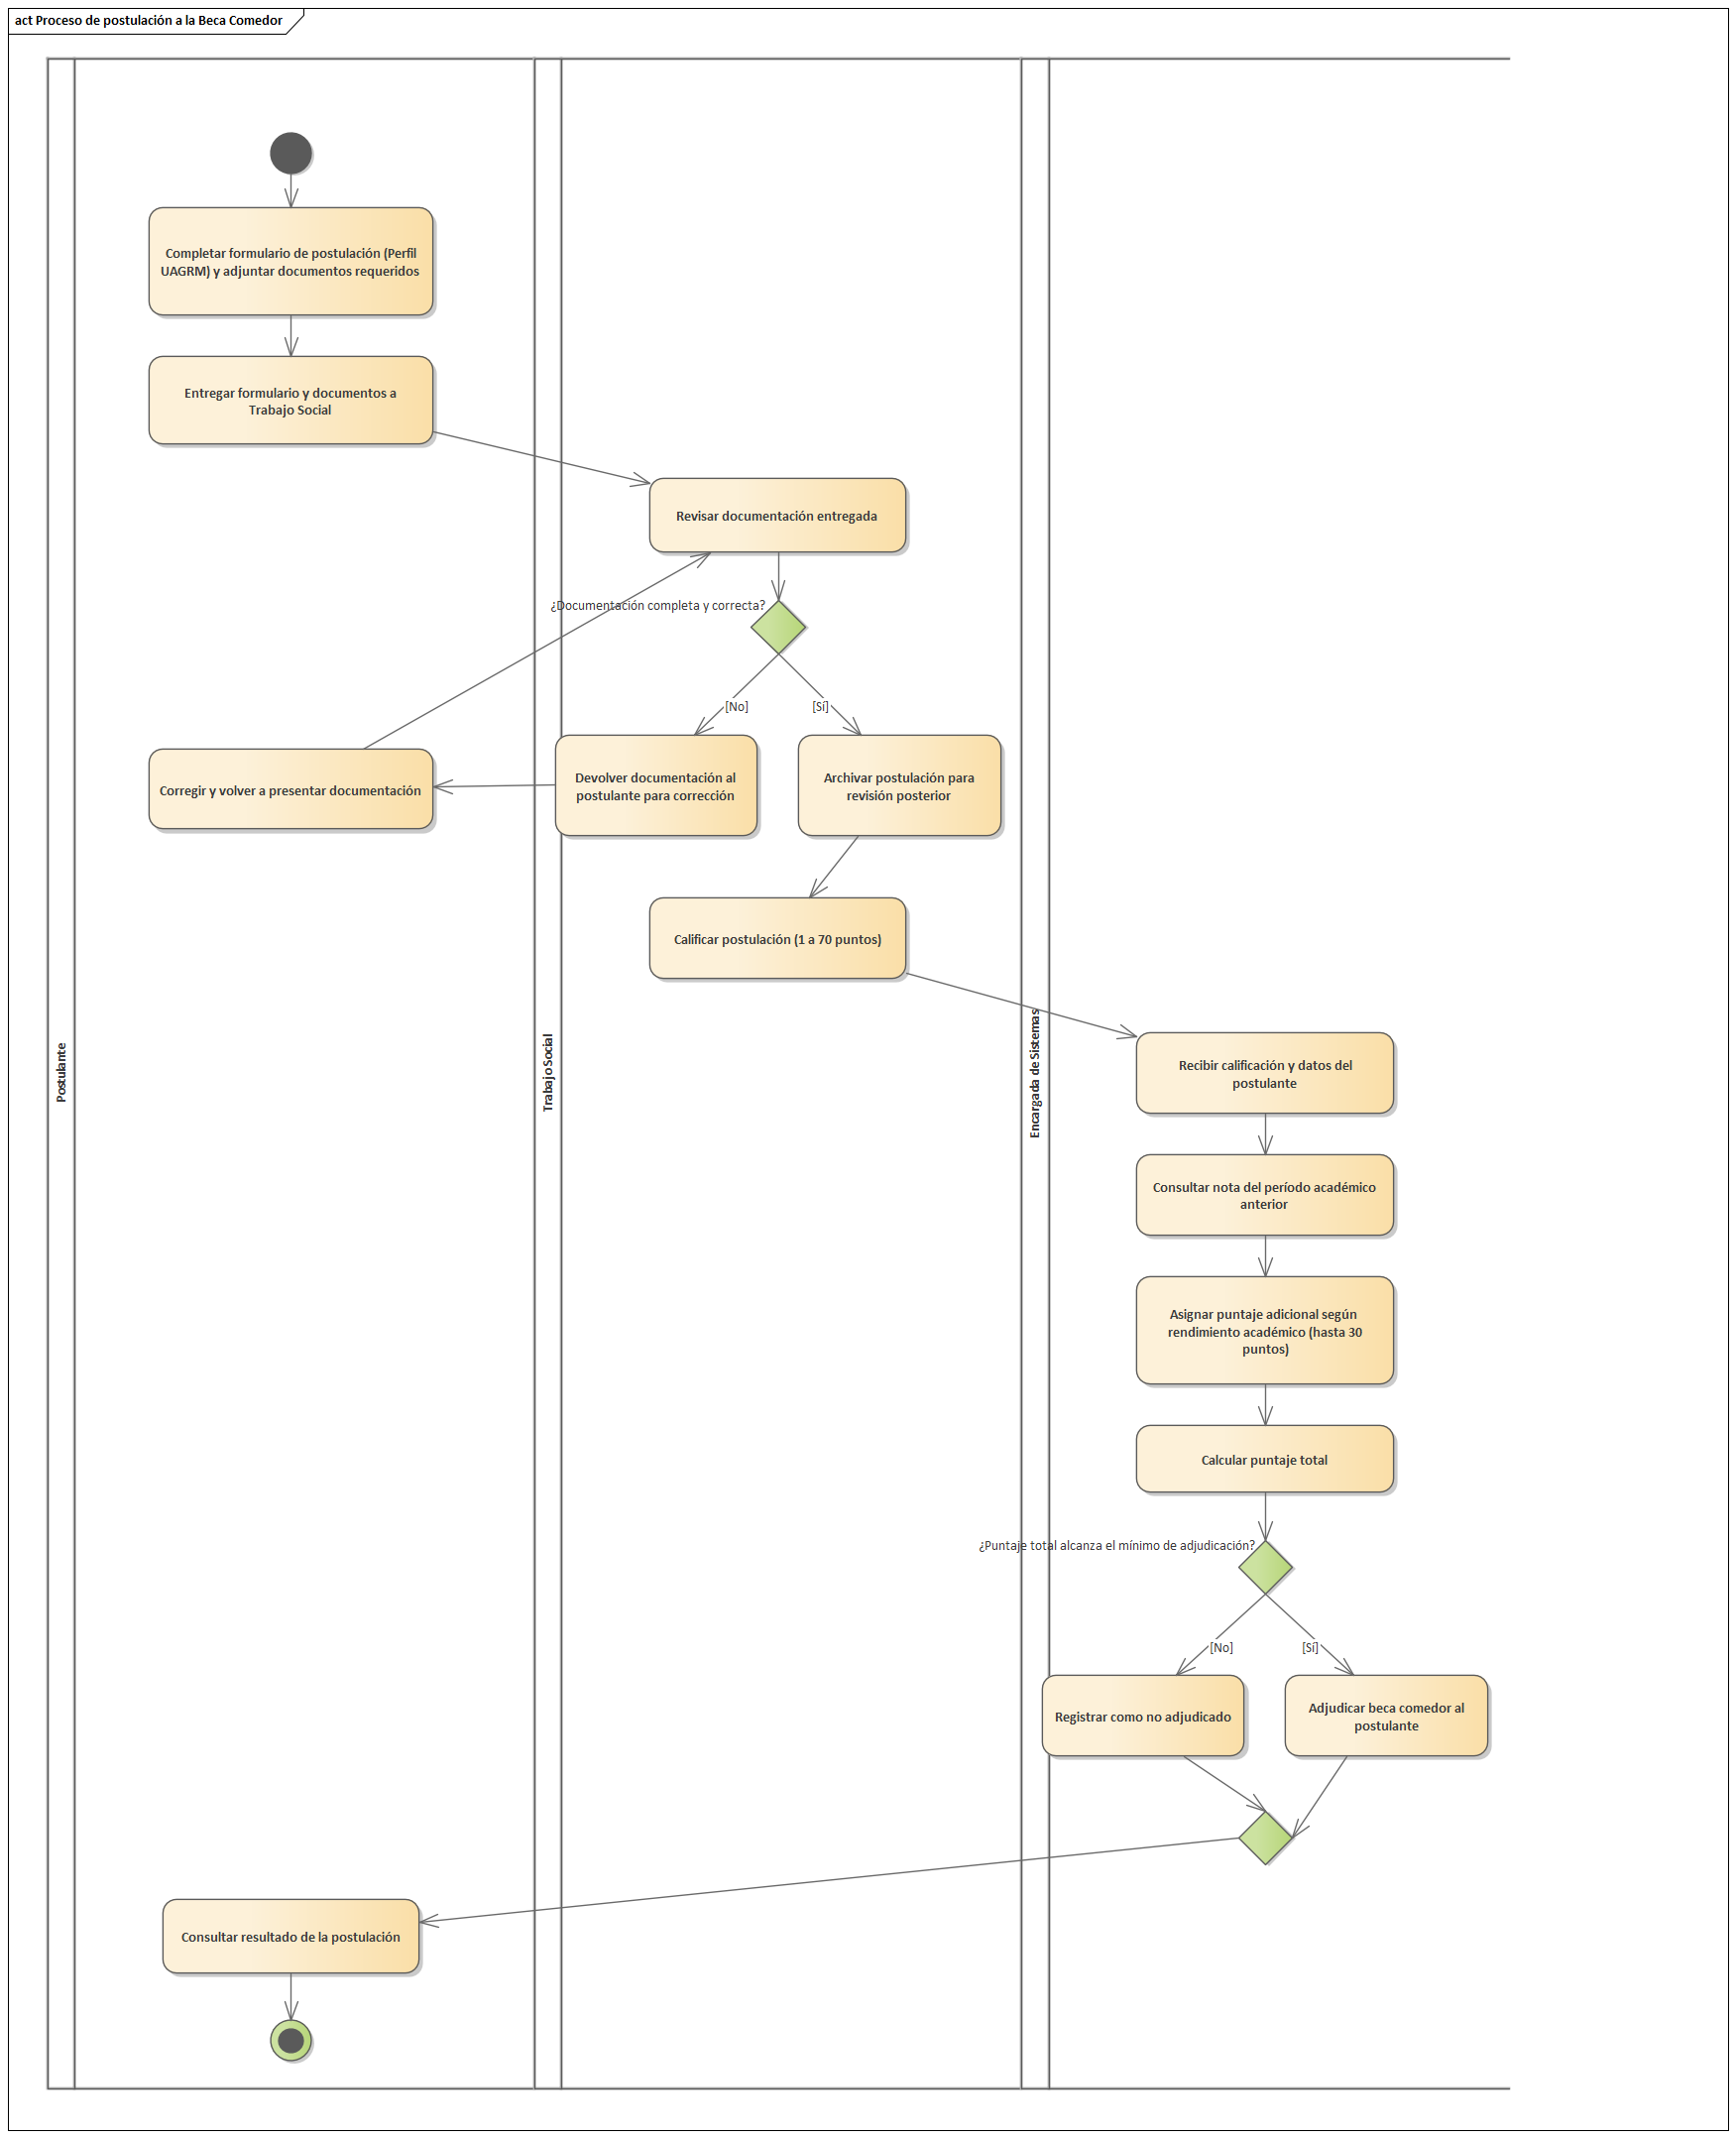
\includegraphics[width=\textwidth,height=0.8\textheight,keepaspectratio]{images/017_Postulacion_Beca.png}

\smallskip
\noindent\raggedright\textit{Nota.} Elaboración propia basado en la entrevista con el personal de la DUBSS.
\end{figure}


\paragraph{3.1.7.2. Datos.}

% [PENDIENTE]: Redactar "Datos".

\paragraph{3.1.7.3. Arquitectura.}

\subparagraph{3.1.7.3.1. Diagrama de despliegue.}

% [PENDIENTE]: Redactar "Diagrama de despliegue".

\subsubsection{3.1.8. Definición de criterios de calidad}

% [PENDIENTE]: Redactar "Definición de criterios de calidad".

\subsubsection{3.1.9. Lista priorizada de casos de uso}

La identificación, priorización y detalle de los casos de uso se desarrolla en las secciones 3.2.5 a 3.2.8.

